\documentclass[a4paper,10pt]{article}

\usepackage{url,color, graphicx, wrapfig}
\usepackage{parskip}
\usepackage{longtable}
\usepackage{verbatim}

% Fix special chars
\usepackage[norsk]{babel}
\usepackage[T1]{fontenc}
\usepackage[utf8]{inputenc}

% Fix links
\usepackage{hyperref}
\definecolor{linkcolour}{rgb}{0.0,0.0,0.0}
\hypersetup{colorlinks,breaklinks,urlcolor=linkcolour, linkcolor=linkcolour}

% Fix headers
\usepackage{titlesec}
\titleformat{\section}{\Large\scshape\raggedright}{}{0em}{}[\titlerule]
\titlespacing{\section}{0pt}{3pt}{3pt}

% Fix margins
\usepackage[width=17cm, left=2cm, top=1.5cm, bottom=1.5cm, a4paper]{geometry}

\begin{document}

\pagestyle{empty} % non-numbered pages

\par{\Huge Gunnar Inge Gjøvik Sortland\bigskip\par}

\begin{wrapfigure}[0]{r}{0.18\textwidth}
  \vskip -2cm
  \vspace{-20pt}
  \begin{center}
    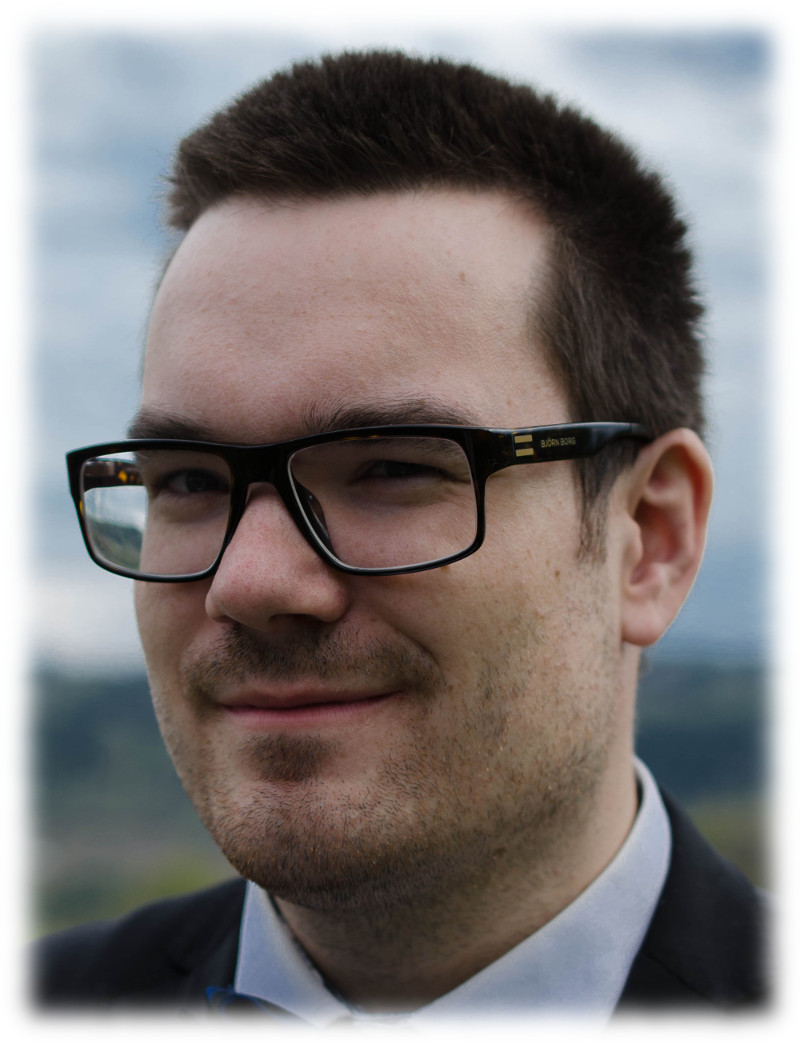
\includegraphics[height=0.15\textheight,keepaspectratio]{me}
  \end{center}
 \vspace{-20pt}
\end{wrapfigure}

\begin{tabular}{rl}
  \textsc{Address:}     & Byåsveien 142D, 7021 Trondheim\\
  \textsc{Phone:}     & 90 65 80 23\\
  \textsc{Email:}       & \href{mailto:gunnaringe@gmail.com}{gunnaringe@gmail.com}\\
  \textsc{Birth:}        & 23. april 1985\\
%  \textsc{Sivilstatus:} & Gift\\
\end{tabular}

\vskip 0.5cm

% ################################################################## %

\section{About me}
Gunnar Inge obtained a Master's Degree (Master of Science /
Sivilingeniør) during the sprint of 2012 at the Norwegian University of Science and Technology
within Computer Science specializing in algorithm and hardware design.

For his thesis he won the FPGA Forum's prize of best master's thesis
within the field of FPGAs. FPGAs are integrated circuits which
contains programmable logic, such that this can be used instead of
printet circuits in tests or areas where there is a need for high
performance and specialized hardware.

During this thesis he developed a fully functional heterogenous multicore architecture processor with a shared memory interface running on an FPGA. To aid development on this architecture a syncronization library was written in C.

For his specialization project he evaluated different Task Based
Parallelism frameworks, such as OpenMP, Intel Cilk Plus and Wool. The
heterogenous multicore architecture developed during the master's
thesis are ment to be expanded into supporting these kind of frameworks.

\begin{comment}
Han har også en bachelorgrad innen samfunnsøkonomi. Gjennom sitt
studie har han også vært aktiv i flere organisasjoner innn politikk,
vært instruktør på en gruppe tilknyttet studentidretten (NTNUI) og
innen den Internasjonale Studentfestivalen i Trondheim
(ISFiT). \newline

Han har erfaring med språk og rammeverk som Java, C/C++, VHDL og
Django/Python. Gjennom sin deltidsjobb har han også erfaring innenfor
storskalasystemer og byggesystemer som Maven. Han jobber hovedsakelig
med Java og C++, men også noe brukergrensesnitt for web ved hjelp av
PHP samt mobile applikasjoner. Han er styremedlem i en
studentidrettsgruppe, hvor han er webansvarlig. Denne webløsningen
inkluderer også all medlemsadministrasjon og er implementert ved hjelp
av Django/Python med bruk av MySQL. \newline

Gjennom sitt engasjement i friville organisasjoner har Gunnar Inge mye
erfaring med teamarbeid. Han har vært aktiv i partipolitisk arbeid, og
har også vært studenttingsrepresentant ved NTNU. I gruppearbeid er han
en aktiv bidragsyter, og er opptatt av å støtte de rundt seg slik at
teamet kan være effektivt og bidra med godt humør. Han har fra sin
deltidsjobb erfaring med bruk av Scrum. \newline
\end{comment}

He is also certified within both frontend development with
HTML5+JavaScript (Programming in HTML5 With JavaScript and CSS3
Specialist) and backend using Java (Oracle Certified Associate, Java
SE 7 Programmer) og C\# (Programming in C\# Specialist).

He is fond of programming and problem solving, and have good
collaboration skills.  He enjoys working both independently and in a
team. He likes to learn, and is a fast learner.  Gunnar Inge is
concerned that the work that is being done is of good quality and
works structured towards that goal.

% ################################################################## %
\section{Education}
\begin{longtable}[l]{rl}	
 \textsc{08.2007--06.2012} & Master of Science i \textsc{Computer Science}, \textbf{NTNU}, Trondheim\\

 \textsc{08.2004--06.2010} & Bachelor i \textsc{Samfunns\o konomi}, \textbf{NTNU}, Trondheim\\

 \textsc{08.2001--06.2004}      & \textbf{Kristelig Videreg\aa ende Tr\o ndelag}, Trondheim\\
 & Specialization in economy and administration, 3FY, 3MX, 2KJ \\
\end{longtable}

% ################################################################## %

\begin{comment}
\section{Key Qualifications}
\end{comment}

% ################################################################## %

\section{Work experience}
\begin{longtable}{r|p{11cm}}

\textsc{08.2012--p.t.} & \textsc{Capgemini Norge AS} \\
& \footnotesize{Consultant} \\

\textsc{06.2011--08.2011} & \textsc{Yahoo! Technologies Norway} \\
& \footnotesize{Summer job} \\

\textsc{01.2011--06.2011} & \textsc{Yahoo! Technologies Norway} \\
& \footnotesize{Part time} \\

\textsc{08.2010--12.2010} & \textsc{Yahoo! Technologies Norway} \\
& \footnotesize{Part time}\\

\textsc{06.2010--08.2010} & \textsc{Yahoo! Technologies Norway} \\
& \footnotesize{Summer job}\\

\textsc{2005--2010} & Kulinarium AS \\
& \footnotesize{Waiter and chef assistant} \\

\textsc{08.2009--12.2009} & \textsc{IDI, NTNU} \\
& \footnotesize{Student assistant TDT4102 -- Procedural and Object-Oriented Programming} \\%Prosedyre- og objektorientert programming, C++} \\

\textsc{08.2009--12.2009} & \textsc{IDI, NTNU} \\
& \footnotesize{Undervisningsassistent TDT4105/TDT4110 -- IT Grunnkurs}\\

\textsc{01.2009--06.2009} & \textsc{IDI, NTNU} \\
& \footnotesize{Studentassistent IT1102 -- IT Grunnkurs}\\

\textsc{08.2008--12.2008} & \textsc{IDI, NTNU} \\
& \footnotesize{Studentassistent TDT4105 -- IT Grunnkurs}\\

\begin{comment}
\textsc{06.2008--08.2008} & \textsc{Buen Helse- og Omsorgssenter} \\
& \footnotesize{Sommervikar}\\

\textsc{15.09.2005--12.2005} & \textsc{Melhus Kommune} \\
& \footnotesize{MOT informatør}\\
\end{comment}
\end{longtable}

% ################################################################## %

\section{Projects}
\begin{longtable}{r|p{11cm}}

\textsc{03.2013--p.t.} & \textsc{Statoil} \\ &
%\footnotesize{\textit{Endur Integration Services-teamet har ansvar for
%  all integrasjon mot Endur i Statoil, som benyttes innenfor
%  gassproduksjon og -handel i Statoil. Da dette er
%  forretningskritiske systemer, hvor feil vil ha store økonomiske
%  implikasjoner, stilles det strenge krav til systemene.
%}
\footnotesize{\textit{The Endur Integration Services-team are
    responsible for all integrations towards Endur in Statoil, used
    within gas production and trade. As this is business critical
    system system, where errors may have severe economical
    implications, these system have strict requirements with regard to
    guaranteed deliveries of messages and monitoring.}
\newline

As a part of this team, Gunnar Inge have developed new integration
modules, introduced unit testing of modules and other required tasks.} \\

\textsc{02.2013--03.2013} & \textsc{Lydia} \\
%& \footnotesize{\textit{Lydia lager et omfattende Facilities Management System, hvor brukere kan administere alle opplysninger som trengs for å drifte en større bygning.}
& \footnotesize{\textit{Lydia delivers a comprehensive Facilities
    Management System, where the system's users can administer all the
    information needed to manage a larger building mass.}
\newline

We developed support for creating reports for rental agreements, with
support for area hatching for usage of the floor plan. The system is developed in .NET 4.0, with use of WPF and Infragistics. This system integrated an existing solution for converting floorplans from AutoCAD format to XAML.} \\

\textsc{09.2012--12.2012} & \textsc{Verdande Technology} \\ &
%\footnotesize{\textit{Verdande Technology AS ble etablert i 2004 av ansatte og
%  studenter fra NTNU i Trondheim. De er verdensledende i utvikling av
%  spesialiserte Case Based Reasoning (CBR) systemer. De leverer
%  programvaretjenester som samler historiske data og hendelser slik at
%  de kan gjenbruke denne informasjonen til å forutse fremtidige
%  hendelser.}
%\newline

\footnotesize{\textit{Verdande Technology AS was established in 2004
    by a group of professors and students from NTNU in Trondheim. They are leading in development of specialized Case Based Reasoning (CBR) systems, delivering software solution for collecting historical data and events. Using this historical data they can extract knowledge which can be used to predict future events and possibly avoid unwanted ones.}
\newline

\begin{comment}
\textit{Deres Edge-plattform er basis for tjenester innen sektorene energi,
finans og helse.Energy benytter denne platformen i DrillEdge, som gir
sanntids besluttningsstøtte for olje-og gasseksperter under borring av
oljebrønner. Ved å samle tidligere erfaring kan systemet gjenkjenne
potensielle fremtidige problemer slik at disse kan unngås slik at
ikke-produktiv tid kan reduseres. Denne løsningen er (per 2012) i bruk
til å overvåke rundt 30 samtidige oljeborringer.}
\newline
\end{comment}

We developed an test client in Java for stress testing an existing real time solution running on the Amazon Elastic Compute Cload (Amazon EC2). The test clients are simulating a typical user session, with configured user behavior.
  \newline

\begin{comment}
Ved bruk av Java API-et til Amazon AWS initierte vi flere
Linux-instanser til å kjøre testklienter for å finne responstid og
oppdateringsrate fra server. Denne informasjonen kan benyttes til å
finne systemets flaskehalser og beregne nødvendig ressursbruk gitt et
visst antall samtidige brukere.
\newline

Stresstestingrammeverket ble organisert som en
master-klient-applikasjon, hvor klientene simulerte en virkelig klient
og master var ansvarlig for alt oppsett og oppstart av klientene og
Amazon EC2 instansene de kjørte på, monitorering av klientene samt å
samle og organisere testdata.
\newline

I prosjektet ble teknologier som Maven, Bamboo og GIT benyttet, og
eksisterende rammeverk som Amazon AWS, SLF4J med Log4J/Logback og
Perf4J ble tatt i bruk. Google Chart API ble benyttet for å
visualisere info. Under hele prosjektet brukte vi Eclipse som
IDE. Prosjektet ble kjørt med Scrum som metodikk, hvor
JIRA/GreenHopper samt Confluence ble benyttet som hjelpemidler.
\end{comment}
} \\
\end{longtable}

%##################

\section{Volunteer duties}
\begin{longtable}{r|p{11cm}}

\textsc{09.2011--09.2012} & \textsc{Sør Trøndelag KrFU} \\
& \footnotesize{2. deputy chairman} \\

\textsc{08.2011--05.2013} & \textsc{NTNUI Tenshi-Tsume} \\
& \footnotesize{Member of board and webadmin (martial arts group)} \\

%\textsc{08.2011--12.2012} & \textsc{NTNUI Tenshi-Tsume} \\
%& \footnotesize{Instruktør (kampsportgruppe)} \\

%\textsc{01.2011--d.d.} & \textsc{Trondheim KrF} \\
%& \footnotesize{Varamedlem til styret} \\

\textsc{02.2010--01.2011} & \textsc{Trondheim Sentrum KrF} \\
& \footnotesize{Chairman} \\

%\textsc{01.2009--02.2010} & \textsc{Trondheim Sentrum KrF} \\
%& \footnotesize{Styremedlem, kasserer} \\

\textsc{11-2008--03.2009} & \textsc{ISFiT -- Student Peace Price} \\
%& \footnotesize{Funksjonær i Studentenes Fredspris} \\
& \footnotesize{Part of the work group of the Student Peace Price} \\

\textsc{2007--2008} & \textsc{Sameiet Brøsetvegen 186} \\
& \footnotesize{Chairman}\\

%\textsc{2007--2008} & \textsc{Borettslaget Boxbo} \\
%& \footnotesize{Nestleder i styret}\\

%\textsc{2007--2008} & NTNUI Judo \\
%& \footnotesize{ Styremedlem} \\

%\textsc{2006--2007} & \textsc{Borettslaget Boxbo} \\
%& \footnotesize{ Styremedlem}\\

\textsc{2006--2007} & \textsc{Studenttinget NTNU} \\
& \footnotesize{ Studenttingsrepresentant }\\

\begin{comment}

\textsc{2005--...} & \textsc{KrFUs studentgruppe i Trondheim} \\
& \footnotesize{ Styremedlem, økonomiansvarlig }\\

\textsc{2005--2008} & \textsc{ Sør-Trøndelag KrFU} \\
& \footnotesize{Styremedlem }\\

\textsc{2005--2006} & \textsc{Melhus PRESS, Redd Barna Ungdom } \\
& \footnotesize{Styremedlem, økonomiansvarlig }\\

\textsc{2005--2005} & \textsc{Melhus PRESS, Redd Barna Ungdom } \\
& \footnotesize{ Leder}\\

\textsc{2004--2005} & \textsc{Melhus PRESS, Redd Barna Ungdom } \\
& \footnotesize{Nestleder, økonomiansvarlig }\\

\textsc{2003--2004} & \textsc{Melhus PRESS, Redd Barna Ungdom } \\
& \footnotesize{Styremedlem }\\

\textsc{2003--2004} & \textsc{Melhus Idrettslag, Volleyballavdelingen } \\
& \footnotesize{Oppmann for 3. divisjonslaget }\\

\textsc{2003--2004} & \textsc{Sør-Trøndelag KrFU } \\
& \footnotesize{ Styremedlem}\\

\textsc{2002--2003} & \textsc{Elevrådet Kristelig Videregående Trønderlag } \\
& \footnotesize{ Nestleder}\\

\textsc{2001--2003} & \textsc{Melhus KrFU } \\
& \footnotesize{ Styremedlem, økonomiansvarlig (2002-2003)}\\

\end{comment}

\end{longtable}

% ################################################################## %

\begin{comment}
\section{Kurs og sertifikater}
\begin{longtable}[l]{rl}
 \textsc{Mai} 2003 & Førerkort -- Klasse B\\
 \textsc{Høst} 2003 & Volleyball -- Trenerkurs 1\\
 \textsc{Vinter} 2002 & Volleyball -- Dommerkurs\\
\end{longtable}
\end{comment}

\begin{comment}
\section{Sertifiseringer}
\textsc{Microsoft}
\begin{longtable}[l]{rlr}
 \textsc{Januar 2013} & Programming in HTML5 with JavaScript and CSS3 Specialist & (70-480) \\
 \textsc{Januar 2013} & Programming in C\# Specialist                             & (70-483) \\
\end{longtable}

\textsc{Oracle}
\begin{longtable}[l]{rlr}
 \textsc{Februar 2013} & Oracle Certified Associate, Java SE 7 Programmer & (1Z0-803 Java SE 7 Programmer I) \\
\end{longtable}
\end{comment}
% ################################################################## %

\begin{comment}
\section{Språk}
\begin{longtable}[l]{rl}
 \textsc{Norsk:}   & Morsmål \\
 \textsc{Engelsk:} & Godt muntlig og skriftlig \\
\end{longtable}
\end{comment}

% ################################################################## %

%\begin{comment}
\section{Programming Languages}
\begin{longtable}[l]{rl}
 \textsc{Java} & Good command \\
 \textsc{C\#} & Good command \\
 \textsc{C/C++} & Good command \\
 \textsc{Python} & Good command \\
 \textsc{JavaScript} & Good command \\
 \textsc{VHDL} & Used for master's thesis \\
 \textsc{Ruby} & Some knowledge \\
 \textsc{Prolog} & Some knowledge \\
 \textsc{Oz} & Some knowledge \\
 \textsc{Assembly} & Some knowledge \\
\end{longtable}
%\end{comment}
% ################################################################## %

\begin{comment}
\section{Interesser}
Liker å programmere. Har interesse for algoritmekonstruksjon og tallteori.
Samfunnsengasjert, med særlig interesse for internasjonal handel og
politikk. Liker å ta bilder. Glad i aktivitet, og liker å holde meg i form.
Ellers liker jeg godt å tilbringe tid med kone og min to måneder gamle datter.
\end{comment}
% ################################################################## %

\begin{comment}
\section{Referanser}
Oppgis ved forespørsel.
\end{comment}

% ################################################################## %

\end{document}
